Dentro del sistema, las predicciones son muy importantes, ya que dependiendo del comportamiento del dispositivo es posible realizar una predicción de cómo será el comportamiento de los recursos de este.
\newline
Para el caso de la predicción con el algoritmo de mínimos cuadrados, primero fue necesario crear un archivo con extensión .rrd, el cual nos ayudará a almacenar el uso de un determinado recurso, así como el promedio de uso del mismo. Una vez creado el archivo, el sistema se encarga de almacenar una colección de datos sobre el uso de ese recurso, para finalmente realizar una predicción sobre cómo será el uso de dicho recurso en el futuro. El código utilizado para la generación del archivo .rrd se muestra a continuación.

\pagebreak
\begin{figure}[htbp!]
	\centering
		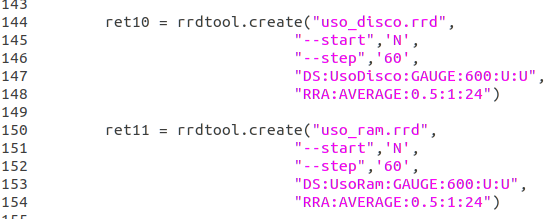
\includegraphics[width=0.8\textwidth]{imagenes/MinimosCuadrados/MinimosCuadradosRRD2.png}
	\caption{Creación del archivo .rrd para capturar la información y aplicar el algoritmo de mínimos cuadrados.}
\end{figure}

Posteriormente, se hizo uso del algoritmo de mínimos cuadrados, para así poder generar una gráfica que nos muestre de qué forma se comportará nuestro dispositivo. En las siguientes imágenes se muestra la forma en que se creó la imagen y la predicción, así como el resultado final tras utilizar este algoritmo.

\begin{figure}[htbp!]
	\centering
		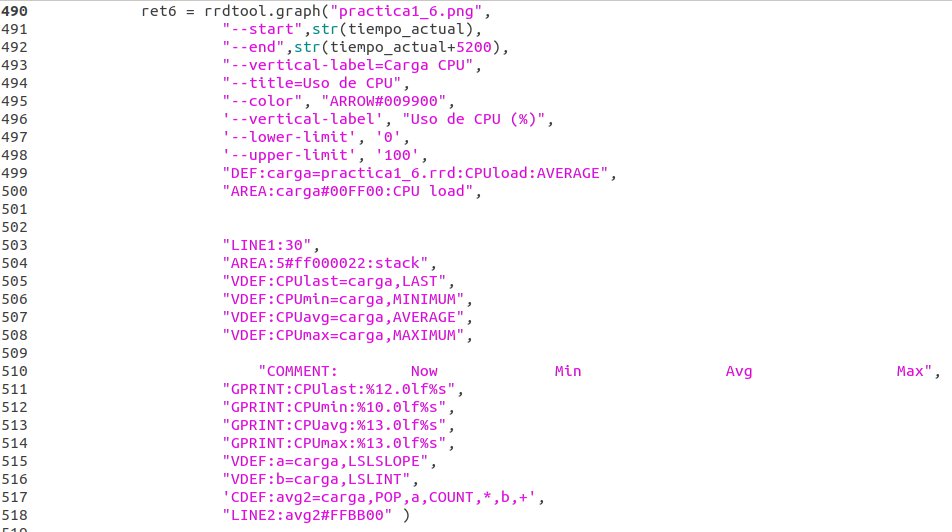
\includegraphics[width=0.8\textwidth]{imagenes/MinimosCuadrados/CreacionImagenMinimosCuadrados.png}
	\caption{Forma de creación de la gráfica de mínimos cuadrados.}
\end{figure}

\pagebreak
\begin{figure}[htbp!]
	\centering
		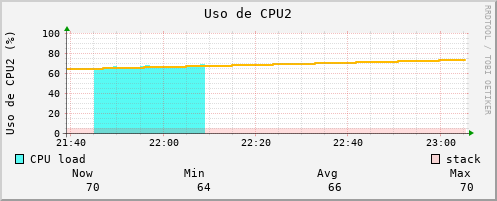
\includegraphics[width=0.8\textwidth]{imagenes/MinimosCuadrados/practica1_7.png}
	\caption{Gráfica generada para el uso del CPU 2.}
\end{figure}

 
